% \subsection{IPS-N Tortuga}

% \begin{center}
%     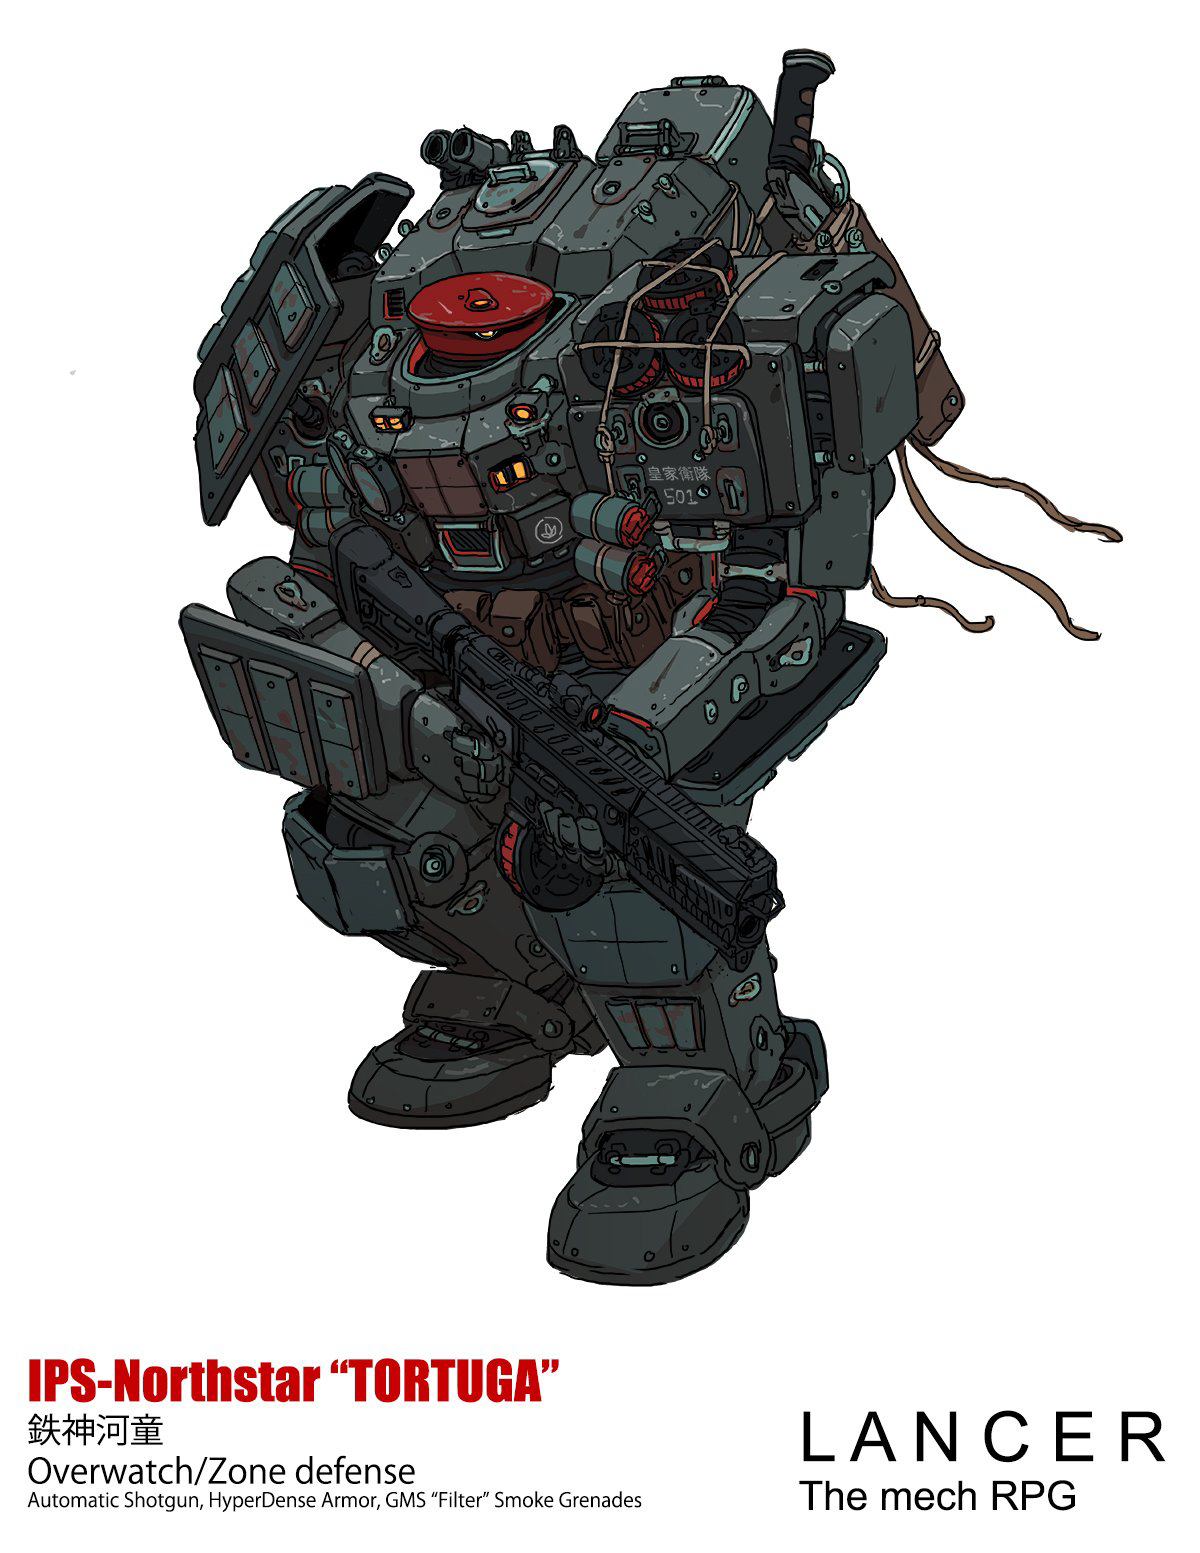
\includegraphics{Tortuga}
% \end{center}

\begin{mech}{IPS-N}{Tortuga}

\fluff{The TORTUGA is IPS-N's short-to-medium range core-line mech. Conceived, tested, and perfected in the void of deep trade space, the TORTUGA is made to breach and clear the spinal columns of capital ships, carriers, and hostile stations. The TORTUGA is built to occupy space, filling hallways with its angular bulk. It defends just as effectively as it attacks, often used in a battering-ram role by boarding parties and ship/stationboard marines. Conversely, the Tortuga is often employed in a defensive posture by marines seeking to repel boarding parties, often using its ablative brachial structures to shield troopers from incoming fire.}

\begin{license}
\item Automatic Shotgun, Siege Ram
\item TORTUGA FRAME, Throughbolt Rounds, Daisy Cutter
\item Pneumatic Hammer, Hyper Dense Armor
\end{license}

\frameBox
[hp = 10,
evasion = 6,
speed = 3,
heat cap = 6,
sensors = 15,
armor = 2,
e-defense = 10,
size = 2,
repair cap = 6,
tech attack = +1,
traits = {\textbf{REFLEX:} The Tortuga gets +1 Accuracy to all overwatch attacks

\textbf{Guardian:} Allied actors adjacent to the Tortuga gain light cover },
sp = 6,
mount one = main mount,
mount two = heavy mount,
core system name = SENTINEL,
core system text = {IPS-N security teams are no strangers to the danger of ship-to-ship or ship-to-station boarding actions. Tight corridors, unstable gravity, dark environments, hard vacuum, and the dual threat of organic and inorganic opposition forces make boarding actions some of the most deadly engagements (by percentage) that one could participate in -- the winning side, according to IPS-N's internal metrics, should expect at least 30\% casualties on average.

To lessen the cognitive burden of pilots and any NHPs or comp/cons they have installed in their chassis, IPS-N developed the SENTINEL co-pilot subsentient partition. The Sentinel is a simple subsentient: a flash-homunculus of an aggregate-intelligence compiled through thousands of after-action reports from boarding actions, debriefings, and volunteer donors. Not a true AI, nor an NHP, the SENTINEL is a robust tactical program similar to a smart weapon, though without the need to cycle it presents certain tactical advantages -- namely, the ability for limited learning and best-guess predictive capabilities alongside its pilot. SENTINELs are largely plain in their personalities, such that they develop, and are a favorite of pilots for their no-nonsense attitude and crisp, efficient counsel.

The SENTINEL is currently under review by a joint USB/UDoJ-HR committee, but no formal stay on production has yet been issued.},
core active name = Hyper-reflex mode,
core active text = {Protocol

For the rest of this combat, your threat with ranged weapons increases to 5 if it was less than 5. You can make one additional overwatch attack between your turns, and any target struck by your overwatch attacks is immediately immobilized until the start of its next turn.
}]


Automatic Shotgun
The IPS-N Deck-Sweeper Automatic Shotgun is a belt-fed scattergun, a favorite of marine pilots aboard stations and capital ships. It's operation is simple and straightforward: charge, point, and fire. The single-barrel constriction allows for pneumatic absorption, dampening the effect of its incredible recoil, and its belt-fed action accepts many types of shot-and-FRAME ammunition.
The DSAS is a mainstay among IPS-N licensed pilots.

Main CQB
Inaccurate
Range 3, Threat 3
2d6 Kinetic Damage

Siege Ram
The Siege Ram is another holdover from IPS-N's pre-merger days. When Bulkheads slam closed and there is a need to get them open, marine pilots mount a siege ram to get the job done. Heavy, dumb, and unbreakable, the Siege Ram is the universal key. Carried in-hand by a qualified chassis, the IPS-N Siege Ram is a solid metal beam with a wedge tip, meant to be slammed into the seam of a sealed bulkhead door and driven home, cracking open ships and stations like a can.

2 SP, Unique

Your ram attacks deal 1d3 kinetic damage on hit. Against stationary objects, deployed cover, terrain, walls, or obstacles, your ram attacks instead deal 10 AP kinetic damage.

Throughbolt Rounds
Throughbolt Rounds are a proprietary IPS-N invention. Throughbolts are Tungsten-jacketed, uranium core rounds with projection-activated plasma sheaths. When fired, the rounds ignite and project a superheated cone of plasma before them, creating a miniature lance effect that ensures multiple-target penetration through soft and hard surfaces.

2 SP
Mod
Choose 1 CQB, cannon, or rifle weapon. When you fire this weapon, draw a line 3 spaces long from your mech, then measure its original range from the end of this line as though the attack was fired from that position (also measure cover and line of sight from this new position for the rest of the attack). This line can easily punch through walls or other barriers. Any targets hit by this line are also hit by the attack. The attack cannot change directions after being fired.

Daisy Cutter
The Daisy Cutter is an effective, if outdated, weapon system for which many marine pilots still place print requisitions. The Daisy Cutter is, essentially, a massive shotgun: the pilot loads a shaped charge into the breech of the Cutter, drops a packed sabot down the barrel, aims, and fires a mixed hellfire cloud of flechette darts, bearings, and ignited magnesium strips, clearing any deck it's been fired on.

Heavy CQB
Limited (1)
Cone 5
3d6 kinetic damage.
The blast cloud from firing this weapon lingers until the end of your next turn, providing light cover to any actor in the affected area.

Pneumatic Hammer
Colloquially known as a `pilebunker', built originally from blast mining equipment, the pneumatic hammer has been refined into a widely feared weapon - a solid-core cylinder cocked and locked in place by a miniaturized gravity well. When fired, the cylinder is propelled forward by a charge of superheated plasma through a cannon-like shaft, creating enormous kinetic force. Without proper reinforcement, the power created by this weapon will literally tear its wielder's arm off.

Main Melee
Loading
Threat 1
1d3+5 kinetic damage
On a Critical Hit with this weapon, your target must pass a hull check or be stunned until the end of its next turn.

Hyper Dense Armor
IPS-N HyperDense Armor is built for use in space. As the name implies, the HyperDense system is forged without respect to the gravitational constraints mechs may face down a gravity well; many pilots flying cores equipped with HyperDense armor are shocked to experience the difference in piloting their mechs down a well versus in the null-gravity of space.

3 SP
Unique, Protocol, 2 heat (self)
You may activate or deactivate this armor system's activation protocols at the start of your turn. While active, it hardens into a shimmering, reflective surface and offers unparalleled protection, granting you resistance to all damage from attacks further away from range 5 of your mech. However, your mech is Slowed while it is active.


\end{mech}
